\section{processIds.c}

	Muestre la pantalla de ejecucución del programa:

	\begin{center}
		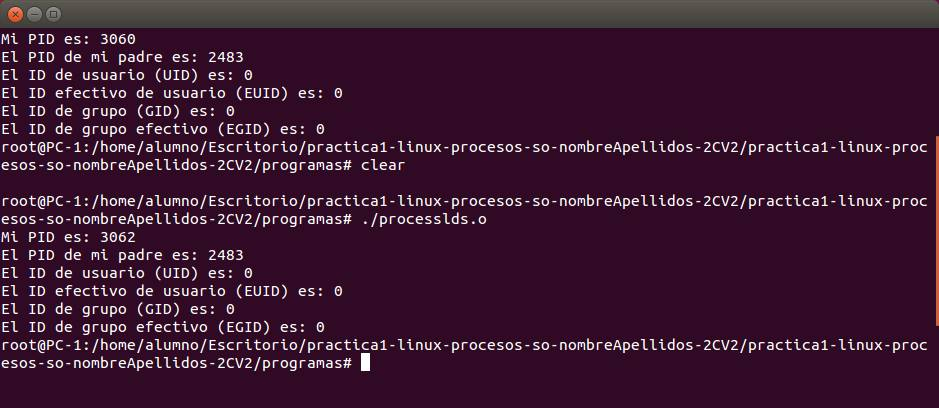
\includegraphics[width=\linewidth]{imagenes/processIDs.png}
	\end{center}

	Describa cuál es el propósito de las siguientes bibliotecas:

	\begin{itemize}

		\item unistd.h\\
		Es el archivo cabecera C/C++ que puentea a varias constantes, tipos y declaraciones de funciones que comprenden el API del sistema operativo POSIX.
		\item sys/types.h\\
		Contiene una lista útiles de tipos incluyendo:
		\begin{itemize}
		\item clock\_t
		\item dev\_t
		\item off\_t
		\item ptrdiff\_t
		\item size\_t
		\item seize\_t
		\item time\_t
		\end{itemize}

	\end{itemize}

	Mencione que representan los siguientes tipos de datos y donde estan definidos:

	\begin{itemize}

		\item pid\_t\\ El tipo de datos pid\_t representa identificadores de proceso.\\ Usted puede obtener el identificador de proceso de un proceso llamando getpid. 
		
		\item uid\_t\\ El tipo de dato uid\_t represmta el indentifcador del usuario.\\ Se puede obtener el identificador con la funcion getuid.
				
		\item gid\_t \\ El tipo de dato gid\_t representa el identificador del grupo.
		\\ Se puede obtener el identificador con la funcion getgid.

	\end{itemize}

	Para las siguientes funciones, mencione dónde están definidas, qué es lo que proporcionan de salida y qué argumentos necesitan de entrada:

	\begin{itemize}

		\item getpid\\ La función getpid devuelve el identificador de proceso del proceso actual.
		\\ Esta definida en unistd.h
		\\ pid\_t getpid(void);
		
		\item getppid
		\\ La función getppid devuelve el identificador de proceso del padre del proceso
		\\ Esta definida en unistd.h
		\\ pid\_t getppid(void);
		
		\item getuid
		\\ La función getpid () devolverá el identificador de usuario real del proceso de llamada.
		\\ La función getpid () siempre será exitoso y sin valor de retorno está reservado para indicar el error.
		\\ Definido en unistd.h
		\\ uid\_t getuid(void);
	
		\item geteuid
		\\ La función geteuid() devolverá el identificador de usuario del proceso en curso.
		\\ La función geteuid() siempre será exitoso y sin valor de retorno está reservado para indicar un error.
		\\ Deefinido en unistd.h
		\\ uid\_t geteuid(void);
		
		\item getgid
		\\ La función getgid () devolverá el ID de grupo real del proceso de llamada.
		\\ La función getgid () siempre será exitoso y sin valor de retorno está reservado para indicar un error.
		\\ Definido en unistd.h
		\\ gid\_t getgid(void); 
		
		\item getegid
		\\ La función getegid () devolverá el ID de grupo efectivo del proceso en curso.
		\\ La función getpid () siempre será exitoso y sin valor de retorno está reservado para indicar un error.
		\\ Definido en unistd.h
		\\ gid\_t getegid(void);
	\end{itemize}
